\documentclass[final]{beamer}

\usepackage[orientation=portrait, size=a0, scale=1.6]{beamerposter} % Use the beamerposter package for laying out the poster
\usepackage{tikz}

\usetheme{Boadilla}

\setbeamercolor{block title}{fg=blue,bg=white} % Colors of the block titles
\setbeamercolor{block body}{fg=black,bg=white} % Colors of the body of blocks
\setbeamercolor{block alerted title}{fg=white,bg=dblue!70} % Colors of the highlighted block titles
\setbeamercolor{block alerted body}{fg=black,bg=dblue!10} % Colors of the body of highlighted blocks


\newlength{\sepwid}
\setlength{\sepwid}{0.024\paperwidth} % Separation width (white space) between columns

%-----------------------------------------------------------

\usepackage{graphicx}  % Required for including images

\usepackage{booktabs} % Top and bottom rules for tables

\begin{document}
\addtobeamertemplate{frametitle}{}{%
	\begin{tikzpicture}[remember picture,overlay]
	\node[anchor=north west,yshift=2pt] at (current page.north west) {
\includegraphics[height=7cm]{LogoISAE.pdf}};
	\end{tikzpicture}}

\addtobeamertemplate{block end}{}{\vspace*{2ex}} % White space under blocks
\addtobeamertemplate{block alerted end}{}{\vspace*{2ex}} % White space under highlighted (alert) blocks

\setlength{\belowcaptionskip}{2ex} % White space under figures
\setlength\belowdisplayshortskip{2ex} % White space under equations

\begin{frame}[t]{\LARGE \hspace{13cm}
Simulation et contrôle des structures thermoélastiques \\ \hspace{13cm} pour des applications spatiales
} % The whole poster is enclosed in one beamer frame

\begin{columns} 
\begin{column}{\sepwid}\end{column} % Empty spacer column

\begin{column}{0.45\textwidth} % The first column
	
\begin{block}{\center PIE 048 \vspace{1cc}}
ISAE Département DISC-DCAS 

Contacts:
\begin{itemize}
\item Andrea Brugnoli \hspace{.5cm} 0750394727 \hspace{.5cm} \href{mailto:andrea.brugnoli@isae.fr}{andrea.brugnoli@isae.fr}
\item Ghislain Haine \hspace{.5cm} ?????????? \hspace{.5cm} \href{mailto:ghislain.haine@isae.fr}{ghislain.haine@isae.fr}
\item Denis Matignon \hspace{.5cm} ?????????? \hspace{.5cm} \href{mailto:denis.matignon@isae.fr}{denis.matignon@isae.fr}
\item Xavier Vasseur \hspace{.5cm} 0561338732 \hspace{.5cm} \href{mailto:xavier.vasseur@isae.fr}{xavier.vasseur@isae.fr}
\end{itemize}

\end{block}

\end{column} 

\begin{column}{0.5\textwidth} % The first column
	\centering
	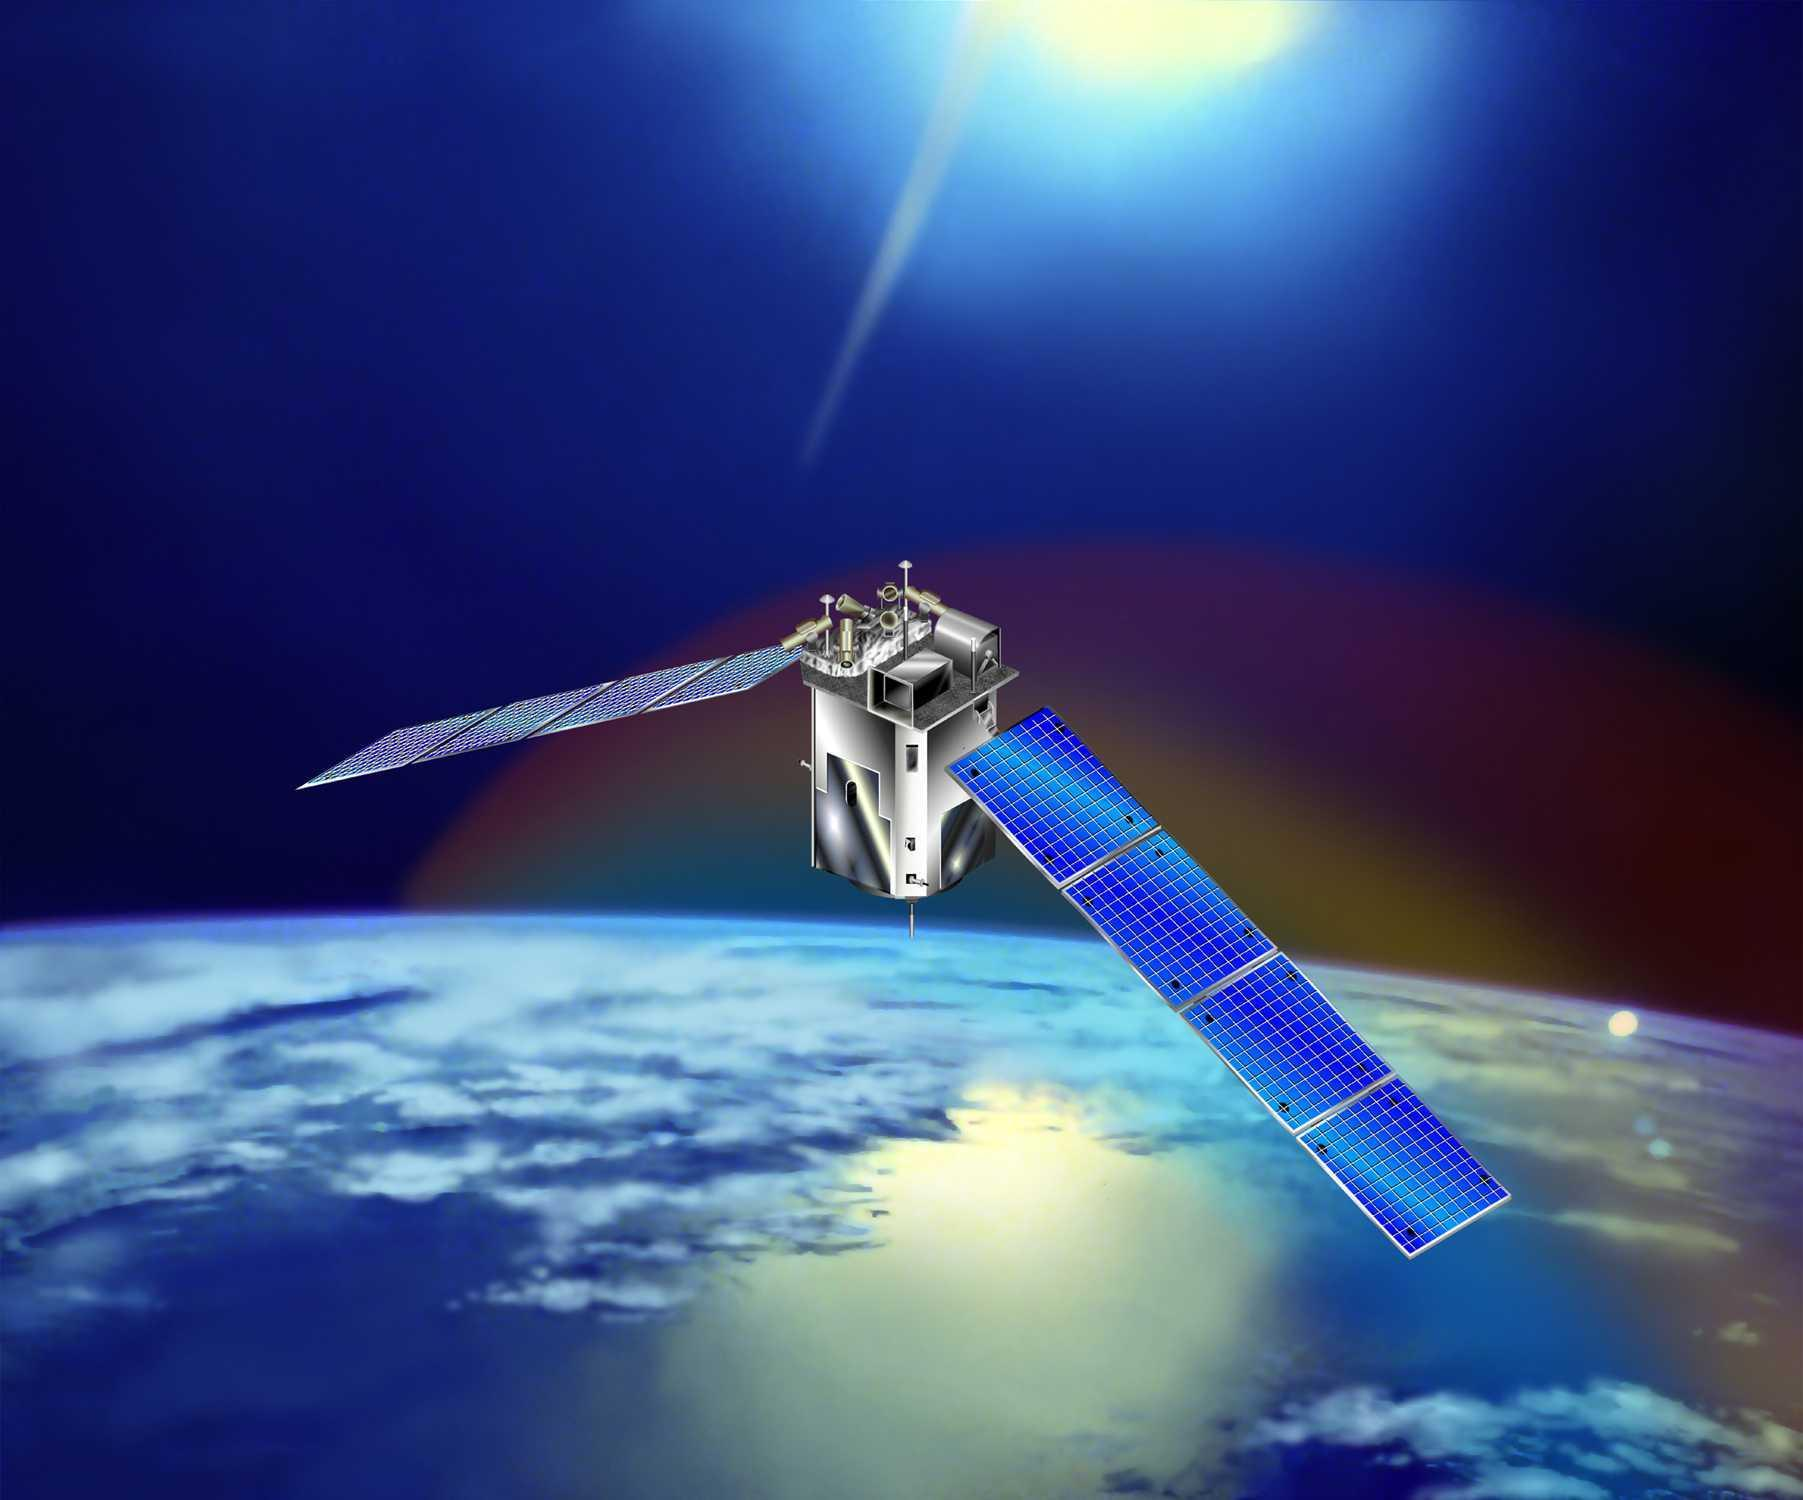
\includegraphics[width=0.75\columnwidth]{satellite.jpg}
\end{column} 

\begin{column}{\sepwid}\end{column} % Empty spacer column

\end{columns}

\begin{columns} 
	
	\begin{column}{\sepwid}\end{column} % Empty spacer column
	
\begin{column}{0.95\textwidth}
\begin{block}{Description et Objectifs \vspace{1cc}}
Dans l'industrie aérospatial l'étude de l'impact thermique sur la partie structurelle à une importance cruciale. Les avions supersonique (le premier Lockheed SR-71 Blackbird datant du 1966)  ont été le premier défi technologique pour le quelle la prise em compte effets thermiques était nécessaire. Le revêtement d'isolation thermique ont été introduit dans la conceptions des turbomachines pour pouvoir résister à des conditions des températures extrêmes. Pour les véhicules spatiaux les systèmes de protection thermique sont indispensables soit pur les opérations en orbite et surtout pour faire face à la rentrée atmosphérique. Le couplage thermoélastique peut aussi induire des micro-vibrations, lorsque un satellite traverse une transition jour/nuit. Les vibrations peuvent affecter la précision du système du pointage, en dégradant les performances. \\

Dans une phase de modélisation préliminaire il est donc importante pouvoir quantifier les efforts l'impact du champs thermique sur la partie structurelle. Pour ça plusieurs approches sont envisageables avec des différent niveaux des complexités:
\begin{itemize}
	\item couplage complet;
	\item problème découple: la production de chaleur du à la déformation mécanique est négligé;
	\item couplage quasi-statique: les termes d'inertie sont négligés mais le couplage est gardé;
	\item problème découplé quasi statique;
	\item problème stationnaire (le problème thermique est donc automatiquement découplé).
\end{itemize}

Dans le cadre de ce projet on s'intéresse à la simulation et au contrôle du problème dynamique thermoélastique à l'aide d'une modélisation port-Hamiltonien. La première étape consistera à formuler le problème thermoélastique comme système port-Hamiltonien en s'appuyant sur des modèles thermoélastique classiques. Il sera en suite important de évaluer l'importance du couplage en comparant le problème couplé et découple. Pour cela des méthodes de discrétisations récentes seront utilisés. L'implémentation numérique s'appuiera sur des libraires existants (FEniCS, Firedrake), qui faciliteront la tache d'obtenir un système discret. Une fois que les modèles discrets seront validés, la réduction du modèle et le contrôle pourront être étudie. \\

\end{block}
\end{column} 

\begin{column}{\sepwid}\end{column} % Empty spacer column

\end{columns}

\begin{columns} 
	\begin{column}{\sepwid}\end{column} % Empty spacer column
	
	\begin{column}{0.95\textwidth}
		\begin{block}{Résultats attendus \vspace{1cc}}
		\begin{itemize}
			\item Une analyse bibliographique,
			\item Une description de la méthodologie et l’analyse mathématique concernant la représentation du couplage,
			\item Un fichier Notebook qui exposera la validité de l’approche proposée,
			\item Un rapport sur le contexte, la méthodologie et les résultats obtenus.
		\end{itemize}
		\end{block}
	\end{column} 
	\begin{column}{\sepwid}\end{column} % Empty spacer column
\end{columns}

\begin{columns} 
	\begin{column}{\sepwid}\end{column} % Empty spacer column
	
	\begin{column}{0.95\textwidth}
		\begin{block}{Compétences attendus \vspace{1cc}}
			\begin{itemize}
				\item Informatique : algorithmique, implémentation sous Python, environnent Unix.
				\item Mathématiques appliquées : Équations aux Dérivées Partielles, Éléments Finis
				\item Mécanique des milieux continus : Principe physique (loi de conservation), \item lois de comportement (fluide \& structure)
			\end{itemize}
		\end{block}
	\end{column} 
	\begin{column}{\sepwid}\end{column} % Empty spacer column
\end{columns}

\end{frame} % End of the enclosing frame

\end{document}
